\section{The Analytical Framework}\label{sec:AnalyticalFramework}

In order to derive an optimal liquidation strategy in a mixed auction market, we must first specify the auction mechanism for each session and how trading will impact the fair price of the market. We consider a market with two trading sessions in succession: a call auction session and a continuous trading session. The mechanism of each session, number of participants in each session and how their interaction affects the price of the underlying risky asset will be described, following by the market impact formula and the optimal liquidation strategy {\color{red} under the risk neutral settings. We then incorporate the risk-aversion factor of a liquidity taker to show the volatility dampening effect of the call auction.}

\subsection{Call auction mechanism and equilibrium price}\label{subsec:AnalyticalFrameworkCallAuction}

In this section we will examine how different participants contribute to the price discovery process during the call auction. We assume the call auction is fully automated, and the matching mechanism is modelled after a Walrasian auction. Specifically, the equilibrium price is determined to maximize the volume traded in the call auction, and therefore has to satisfy the following requirements:

\begin{itemize}
  \item All buy/sell orders at prices higher/lower than the equilibrium price must be executed.
  \item At the execution price, the entire either buy or sell quantity must be matched.
\end{itemize}

Traders can submit and amend orders anytime during the call auction. Those orders are not matched immediately, and placed into the book as "crossed", that is, the highest buy price is higher than the lowest sell price in the book (see Table (\ref{itayoseTable1}) for an example book during the call auction). At the end of the auction period, the orders in the book are matched based on an equilibrium price calculated by the exchange. Table (\ref{itayoseTable2}) gives an example of how a book can be "un-crossed" at the end of the call auctions. All the orders that are unmatched at the end of the call auction will be transferred to the continuous trading session. There is no specialist who can step in to modify the equilibrium price.

\begin{table}[]
  \centering
  \begin{tabular}{c|c|c|c|c}
    \hline
    \textbf{Total Buy} & \textbf{Buy} & \textbf{Price} & \textbf{Sell} & \textbf{Total Sell} \\ \hline
                       &              & 56             & 4000          & 16100               \\ \hline
                       &              & 55             & 10000         & 12100               \\ \hline
    3000               & 3000         & 54             & 2000          & 2100                \\ \hline
    3100               & 100          & 53             & 100           & 100                 \\ \hline
    7100               & 4000         & 52             &               &                     \\ \hline
    10100              & 3000         & 53             &               &                     \\ \hline
  \end{tabular}

  \caption{A sample crossed orderbook during call auction. The orders will be matched at the equilibrium price of 54, which results in 2100 shares traded.}
  \label{itayoseTable1}
\end{table}


\begin{table}[]
  \centering
  \begin{tabular}{c|c|c|c}
    \hline
    \textbf{Buy} & \textbf{Price} & \textbf{Sell} & \textbf{Trade} \\ \hline
                 & 56             & 4000          &                \\ \hline
                 & 55             & 10000         &                \\ \hline
    900          & 54             &               & 2100           \\ \hline
    100          & 53             &               &                \\ \hline
    4000         & 52             &               &                \\ \hline
    3000         & 53             &               &                \\ \hline
  \end{tabular}
  \caption{A sample orderbook at the end of the call auction.}
  \label{itayoseTable2}
\end{table}

We assume that there are two types of participants:

\begin{itemize}
  \item Market markers are those with private information about the value of the asset. This information is not necessary from possessing some insider knowledge about the asset, but from having access to superior information regarding the order flow of the book, such as real-time trades and quotes provided by the exchange and better data processing capability.
  \item Liquidity traders are those without private information and simply want to execute their orders. We assume the demands of liquidity traders are exogenous, and they trade using market orders.
\end{itemize}

Unlike (\cite{Madhavan2015}), we do not assume that there is a specialist setting the equilibrium price, as most exchanges around the world has adopted automated call auction mechanism at the time of this writing\footnote{This mechanism is adopted for the opening call auctions in Singapore Stock Exchange (SGX), Tokyo Stock Exchange (TSE) and Nasdaq Stock Market (NASDAQ). New York Stock Exchange (NYSE) is different, in which a specialist sets the equilibrium price that is not necessarily the same as the volume-maximizing Walrasian price.}. We also do not assume that there are informed traders with information advantage, but a market maker who holds private information and make the market instead. There are several reasons for this setup:
\begin{itemize}
  \item The model setup assumes that, in order to fully utilize the information advantage, the participant who holds it must have the ability to reprice his orders immediately after he receives a new signal. As we assume the private information is mainly from observing the order flow of the book, it means the participant is a high frequency trader (HFT), who can act immediately after each change in market order flow.
  \item There are evidences that a significant portion of high frequency trading during is for liquidity provision. (\cite{Menkveld2013}) studied the trading activity in Chi-X Europe, and found that a majority of high frequency trading activities is market making. Similarly, \cite{Bellia2017} found that there is a correlation between low-latency trading and the subsequent liquidity provision in the call auction in Tokyo Stock Exchange (TSE).
\end{itemize}

We further assume that there is a single market maker who makes the market for $K$ liquidity traders. This can be either a designated market maker obligated to provide liquidity for the market, or an external agent who wants to capture the liquidity premium of the call auction. The market maker is then assumed to have a negative exponential expected utility function of the form
\[
  u(W_e) = -e^{-\lambda W_e}
\]
where $W$ is the terminal wealth of the trader at the end of the call auction. The terminal wealth of the market maker is
\[
  W_e = p_0 (q + e_e) + (c_e - p_e q)
\]
The notions are
\begin{itemize}
  \item $\lambda>0$ is the risk aversion factor of the market maker.
  \item $p_0$ is the stock's fair price at the end of the call auction.
  \item $p_e$ is the stock's equilibrium price at the end of the call auction.
  \item $c_e$ is the initial cash position of the market maker.
  \item $e_e$ is the overnight position of the market maker.
  \item $q$ is number of shares purchased by the market maker at the end of the call auction.
\end{itemize}
To model the asset price at the end of the call auction, we assume that the asset value $p_0$ follows normal distribution with mean $\mu_e$ and precision (the inverse of the variance) $\zeta_e$ \footnote{While this means the stock may have negative price as time goes by, we can ignore this risk as we only need to account for one day of variance. Using an arithmetic stock price process instead of the classical logarihmic price process simplifies other calculation later in the study.}. The private information of market maker $\omega_e$ is then the normal variable
\[
  \omega_e \sim N(p_0, \frac{1}{\psi_e})
\]
The posterior distribution of the asset according to market maker's information set $\Omega_e$ is then normally distributed with mean
\[
  p_0=E[p_0|\Omega_e]=\mu_e \alpha_e + \omega_e(1 - \alpha_e)
\]
where
\[
  \alpha_e = \frac{\zeta_e}{\zeta_e+\psi_e}
\]
and variance
\[
  \sigma_e^2=var[p_0|\Omega_e]=\frac{1}{\zeta_e+\psi_e}
\]
Maximizing expected utility of the market maker, we have the amount of shares submitted at price $p$
\begin{equation}\label{eqn:mm_eval_eqb}
  q(p) = a_e - b_e p
\end{equation}
where $a_e = \frac{p_0}{\lambda \sigma_e^2} - e_e$ and $b_e=\frac{1}{\lambda \sigma_e^2}$. We assume the $K$ liquidity traders will submit a total of $\sum_{i=1}^K x_i$ shares into the call auction to be matched, with negative values implying selling and vice versa. The total shares transacted at a given price $p$ is then
\[
  Q(p) = (p_0 - p) b_e + \sum_{i=1}^K x_i
\]
At equilibrium, we set $Q(p)=0$. This gives the Walrasian price as the matching price at the end of the call auction
\begin{equation}\label{markup_px_eqb}
  p_e = p_0 + \frac{\sum_{i=1}^K x_i}{b_e}
\end{equation}
The matching price is the fair price of the stock with a mark-up in proportion to the supply-demand imbalance in the market. The pricing function is plotted in Figure (\ref{fig:mm_pricing_auction}), which we will use to price our market impact of trading with the call auction in subsection (\ref{subsec:AnalyticalFrameworkTransitionPeriod}) after we examine the continuous trading phase in the next section.

\begin{figure}[h]
  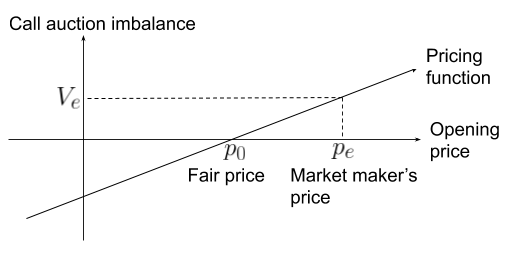
\includegraphics[width=\textwidth]{images/MMPricing}
  \caption{Pricing function of the market maker w.r.t call auction imbalance. If the imbalance is negative, implying that the sell demand is higher than buy demand, the market maker will price the opening price to be lower than his fair price, and vice versa. The slope of the pricing function is $\frac{1}{b_e}$ in Equation (\ref{markup_px_eqb}). $V_e$ is the imbalance at the end of the call auction, while $p_e$ is the opening price. }
  \label{fig:mm_pricing_auction}
\end{figure}

\subsection{Continuous auction mechanism and agents' behaviours}\label{subsec:AnalyticalFrameworkContinuousAuction}
During the continuous trading session, orders can be posted into the market at anytime during the session to be matched. If a buy order has a price that is higher than the current lowest offer in the book, it will be matched immediately, and vice versa for a sell order. Otherwise, it will be added into the book.

Similar to the call auction, we model the continuous auction as a multi-round two-stage game. At the beginning of each round, we pick randomly a liquidity trader to act as the counterparty of the market maker. In the first stage of the round, the market maker places limit orders in the book according to his risk tolerance and private information. In the second stage, the liquidity trader will place a market order based on his exogenous demand. This setup is slightly different from the call auction in which:
\begin{itemize}
  \item Unlike the call auction, only the market maker can submit limit orders during the first stage of the game. He has no knowledge of the liquidity trader's order, and only submit orders based on his own evaluation of the asset's value.
  \item The liquidity trader can only submit market orders during the final stage of the game, after the market maker has finished layering his orders in the book.
\end{itemize}
Under this mechanism, the market maker has a speed advantage with respect to the rest of the market, since he can evaluate the current fair pricing of the asset after each trade. After the reevaluation, he can modify his orders in the market to reflect the updated belief before any liquidity traders can place a new order. This grants the market maker distinct competitive advantage, in the sense that he can reprice his orders in the book before getting hit by any adverse selection event. This gives incentive to market makers to perform high frequency trading.

Similar to the call auction, we assume the market maker has private information about the asset from his superior analytical capability. Again, let assume the immediate asset value at the end of the continuous auction's round is a random variable $v_c$ normally distributed with mean $\mu_c$ and precision $\zeta_c$. The market maker deduces his own evaluation with a private signal
\[
  \omega_c \sim N(v_c, \frac{1}{\zeta_c})
\]
and forms a posterior belief on the asset value at the end of the round as a normal random variable with mean
\[
  v_c=\mu_c \alpha_c + \omega_c(1 - \alpha_c)
\]
where
\[
  \alpha_c = \frac{\zeta_c}{\zeta_c+\psi_c}
\]
and variance
\[
  \sigma_c^2=\frac{1}{\zeta_c+\psi_c}
\]

At the beginning of each round, the market maker has a position $e_c$ that he wants to liquidate. Maximizing the market maker's utility function, we have his order quantity function in the book:
\begin{equation}\label{eqn:mm_eval_cont}
  q_c(p) = a_c - b_c p_c
\end{equation}
where $a_c = \frac{v_c}{\lambda \sigma_c^2} - e_c$ and $b_c=\frac{1}{\lambda \sigma_c^2}$. Let assume the liquidity trader needs to transact $y_0$ shares. The average price he gets after submitting his market order is
\[
  p_{c0} = \frac{a_c-y_0}{b_c} = p_0 - \frac{1}{b_c} y_0
\]
where
\[
  p_0 = \frac{a_c}{b_c}
\]
is the best price quoted by the market maker. Note that the position is from the perspective of the market maker, that is, the higher number of shares the liquidity trader wants to buy, the higher markup price he will have to pay to transact immediately. In other words, the markup price that the liquidity trader receives is
\begin{equation}\label{eqn:markup_px_cont}
  p_{c0} = p_0 + \frac{1}{b_c} y_0
\end{equation}

Comparing Equation (\ref{markup_px_eqb}) and Equation (\ref{eqn:markup_px_cont}), we can see that, ceteris paribus, the instantaneous market impact of trading during the auction phase has a higher chance of getting offset by other liquidity traders in the market. On the other hand, during the continuous phase, the liquidity trader will always receive an adverse markup price implied in market maker's quotes. This is clearer once we examine the transition period immediate after market opening in the next subsection.

\subsection{Price discovery at market opening}\label{subsec:AnalyticalFrameworkTransitionPeriod}

There is empirical evidence that the transition period immediate after market opening is crucial in determining the effectiveness of the opening call auction (\cite{Pagano2013}). In this subsection, we analyze how the market maker, and consequently the spread, may behave during this period, and the subsequent effects on the liquidity trader. Recalling from Equation (\ref{markup_px_eqb}), the opening price is marked up proportional to the buy-sell imbalance at the end of call auction. Let
\[
  V_e = \sum_{i=1}^K x_i
\]
be the imbalance at the end of call auction. Based on the imbalance, the market maker will provide the liquidity necessary for the market to open at equilibrium price
\[
  p_e = p_0 + \frac{V_e}{b_e}
\]
Without loss of generality, let $V_e$ be positive, implying that the market has more buy interests than sell interests. During the call auction, the market maker will sell $V_e$ shares at price $p_e$ higher than his estimated fair value of $p_0$, and has an unrealized gain of
\[
  G_e = (p_e - p_0) * V_e
\]
To capitalize this gain after market opening, the market maker will need to make a spread. Continuing from the call auction's we have the pricing function of the market maker during this period:
\[
  q(p) = a_e - b_e p
\]
where $a_e = \frac{p_0}{\lambda \sigma_e^2} - V_e$ and $b_e=\frac{1}{\lambda \sigma_e^2}$, based on his signal when pricing the call auction. As $V_e$ is positive, this implies that the market maker is willing to sell at $p_e$, {\color{red} the opening matching price after the call auction}. On the other hand, it is reasonable to assume that he will want to liquidate his position acquired from the opening call auction at $p_0$, his fair price of the asset at the end of the call auction. Therefore, the market maker will make a spread of $\frac{V_e}{b_e}$ immediately after call auction. The quotes of the market maker {\color{red} in this scenario} are illustrated in Figure (\ref{fig:mm_pricing_transition}).

\begin{figure}[h]
  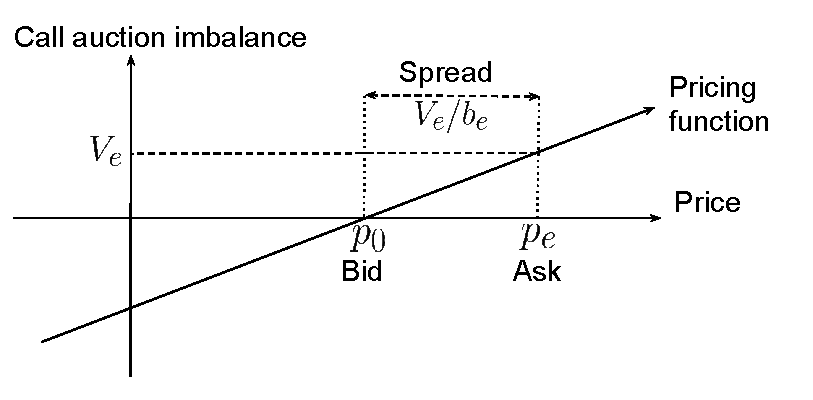
\includegraphics[width=\textwidth]{images/MMPricingTransition}
  \caption{Market maker's quotes immediately after opening w.r.t call auction imbalance {\color{red} as described in Subsection (\ref{subsec:AnalyticalFrameworkTransitionPeriod})}. Upon market opening, the market maker will short $V_e$ shares at $p_e$. His evaluation of the asset's fair value is at $p_0$. {\color{red}To capitalize his gains}, he will quote the ask side further away at $p_e$, and bid side at $p_0$. The bid-ask spread is then $\frac{V_e}{b_e}$, based on the market maker's pricing function (\ref{eqn:markup_px_cont}).}
  \label{fig:mm_pricing_transition}
\end{figure}

Interestingly, the bid-ask spread after market opens reveals the market maker's pricing in the call
auction, as we can calculate the implicit factor $b_e$ as
\begin{equation}\label{eqn:expected_spread}
  b_e = \frac{V_e}{\zeta_e}
\end{equation}
where
\begin{itemize}
  \item $V_e$ is the matching volume at the open of continuous trading session.
  \item $\zeta_e$ is the spread at the open of continuous trading session.
\end{itemize}

From the similarity of the pricing function during the call auction in Equation (\ref{markup_px_eqb}) and the continuous auction in Equation (\ref{eqn:markup_px_cont}), we can see that, ceteris paribus, it is advantageous to trade in both sessions to consume liquidity from both to lower his market impact. This will be clearer once we derive the optimal trading strategy in the next section. Moreover, as the call auction compresses the liquidity over a long period of time in one single price, there is usually a much larger quantity traded than an average market order during continuous auction. Consequently, the market marker will need to unwind the position acquired from the call auction over a transition period immediately after the matching. This will affect the pricing for the liquidity trader during the continuous auction period, in addition to the normal pricing in the continuous session. Specifically, the liquidity trader will potentially face one of the following two scenarios during the call auction:

\begin{itemize}
  \item {\textbf{Scenario 1: The liquidity trader trades in the same direction as the market imbalance}
        As $V_e$, the buy-sell imbalance at the end of the call auction, is assumed to be positive, we have the liquidity trader wants to buy in this case. As a result, his block trade size of $\nu$ will push the opening ask up, from $p_e$ to $p_e^+$
        \[
          p_e^+ =  p_0 + \frac{V_e + \nu}{b_e}
        \]
        As he is buying, this is equivalent to lifting the offer during the continuous phase. In this case, ceteris paribus, there is no difference between trading during the auction and trading during the continuous phase.
        }
  \item {
        \textbf{Scenario 2: The liquidity trader trades against the market imbalance}
        In this case, the liquidity trader will sell to the market, similar to the market maker. Therefore, he is providing liquidity to the market, reducing the bid-ask spread immediately after market opening. Consequently, the opening price bid will improve from $p_e$ to $p_e^-$
        \[
          p_e^- = p_0 + \frac{V_e - \nu}{b_e}
        \]
        As he is selling, this is equivalent to placing his offer into the bid-ask spread during the continuous phase and getting filled immediately.
        }
\end{itemize}

\begin{figure}[h]
  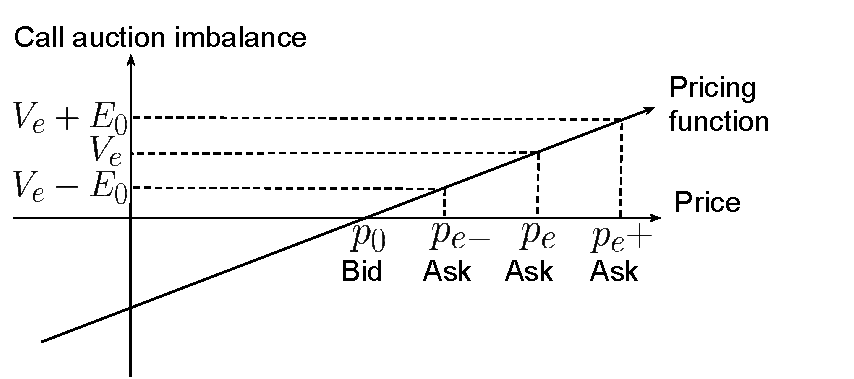
\includegraphics[width=\textwidth]{images/MMPricingTransitionPeriod}
  \caption{Bid-ask spread during the transition period}
  \label{fig:mm_pricing_transition_period}
\end{figure}

As the market maker is buying at the fair price of $p_0$ and selling at a discounted price $p_e$, it is reasonable to assume that he will get filled more on the bid side than the ask side {\color{red} (Need more justifications here, based on market order flow at open)}. This allows the market maker to reduce his inventory over time, and therefore tighten the bid-ask spread. Depending on which scenario the liquidity trader falls into, the market maker's behaviour may affect his cost of liquidation. Specifically, we have:

\begin{itemize}
  \item Under Scenario 1, trading in the call auction results in an ongoing penalty cost to the liquidity trader that will decay over time, as he will need to lift the offer to buy. Let the speed of liquidation of the market maker be $\rho$ and $V_t$ be the remaining position of the market maker acquired from the call auction in Scenario 1. Consequently, we have
        \[
          dV_t = -\rho V_t
        \]
        \[
          V_t[0]=(V_e + \nu)
        \]
        \begin{equation}\label{eqn:recovery_term_eqb}
          \Leftrightarrow V_t = (V_e + \nu) e^{-\rho t}
        \end{equation}
        where $\nu$ is the liquidity trader's block trade size during auction. The resulting spread due to our trading during the call auction at time $t$ will be
        \[
          \zeta_t = \frac{e^{-\rho t}}{b_e}  (V_e + \nu)
        \]
        Therefore, we would expect the spread to be wide initially, and slowly narrowing due to the inventory management effects from the market maker. This is in agreement with current empirical evidence that the bid-ask spread narrows shortly after market opens.
  \item Under Scenario 2, trading in the call auction has no "spillover" effect on the liquidity trader, as the liquidity trader will keep hitting the bid to sell while the market maker will try to improve the offer.
\end{itemize}

This "spillover" cost only incurs half of the time, under Scenario 1, while under Scenario 2 there is no additional cost for the liquidity trader during the continuous phase. Assuming both scenarios are equally likely, the expected markup cost to the liquidity trader during this transition period is:

\begin{equation}\label{resilence_term}
  \zeta_t = \frac{e^{-\rho t}}{2 b_e}  (V_e + \nu)
\end{equation}
which we use in the next section to derive the optimal liquidation strategy for the liquidity trader.

\subsection{Optimal liquidation strategy in a mixed auction market}

Based on the behaviors of market makers in the previous subsections, we can derive the market impact of trading for the liquidity trader across the sessions. Let the fundamental price process $S_t$ at time $t$ be
\[
  S_t = S_0 + \int_0^t \sigma dZ_s
\]
that is, $S_t$ follows a classical arithmetic random walk without any drift. The actual price process $P_t$ is then the combination of the fundamental price process $S_t$ and a short term deviation process $D_t$ due to the market maker repricing his book, as described in Subsection (\ref{subsec:AnalyticalFrameworkCallAuction}) and (\ref{subsec:AnalyticalFrameworkContinuousAuction}):

\[
  P_t = S_t + D_t
\]

From Equation (\ref{markup_px_eqb}) and Equation (\ref{eqn:markup_px_cont}), we can add into $D_t$ a linear cost component proportional to the trading sizes under each session:
\begin{equation}\label{short_term_deviation}
  D_t = \alpha \nu + \xi(t) \beta
\end{equation}
where
\begin{itemize}
  \item $\nu$ is the block trade size at the end of the call auction
  \item $\xi(t)$ is the continuous trading rate of the liquidity trader
  \item $\alpha$ and $\beta$ are the cost penalty factor for aggressing the book during the call auction and continuous auction, respectively. We have $\alpha=\frac{1}{b_e}$ and $\beta=\frac{1}{b_c}$ based on Equation (\ref{markup_px_eqb}) and Equation (\ref{eqn:markup_px_cont}), respectively.
\end{itemize}
Equation (\ref{short_term_deviation}) is similar to what has been described as the "temporary impact" term in in the pioneering works of \cite{BertimasLo1999} and \cite{Almgren2000}. On the other hand, from Equation (\ref{resilence_term}), we have the expected spillover cost of trading during call auction to continuous phase is:
\[
  R_t = \frac{\alpha (\nu + \bar{V_e}) e^{-\rho t}}{2}
\]

The short term deviation term $D_t$ is then
\[
  D_t = \underbrace{\alpha \nu }_\text{Cost of the call auction} +
  \underbrace{\frac{\alpha (\nu + \bar{V_e}) e^{-\rho t}}{2}}_\text{Spillover cost} +  \underbrace{\beta \xi(t)}_\text{Cost of the continuous auction}
\]
and the execution cost is
\begin{equation}\label{eqn:cost_equation_all}
  C_t = \alpha \nu^2 + \frac{\alpha (\nu + \bar{V_e})}{2} \int_0^t e^{-\rho t} \xi(s) ds + \beta \int_0^t \xi(s)^2 ds
\end{equation}

Based on the execution cost equation, we can derive an optimal strategy for the liquidity trader. {\color{red} We first assume that the trader is risk-neutral with respect to the volatility of the market during trading phase, to show the relevance of the call auction in trading cost reduction. We then examine the optimal trading strategy under risk-aversion, to show the variance dampening effect of the call auction.}

\subsubsection{Optimal trading strategy under risk-neutral setting}\label{sec:risk_neutral_opt_strat}

Let assume the liquidity trader wants to unwind a large position, and he has the option to execute his trades in both the call auction and the continuous auction. We have the following notations regarding his trading strategy:

\begin{itemize}
  \item $Q_t$ is the total number of shares of his portfolio at time t.
  \item $\xi(t)$ is the continuous liquidation strategy during the continuous trading auction.
  \item $\Xi(t)=\int_0^t \xi(s) ds$ is the number of total executed shares at time $t$.
  \item $\nu=x_0 - \int_0^T \xi(s) ds$ is the size of the block trade shares executed at the end of the opening call auction.
\end{itemize}

Based on the Proof (\ref{proof:optimal-strategy-mixed-auction}) in the Appendix, we have the optimal size of block trade in the call auction as:
\[
  \nu = \frac{x_0 F_{11} + V_e F_{12}}{F_2}
\]
where
\[
  F_{11} = 8 e^{T \rho} \beta \rho [\alpha - e^{T \rho} (\alpha - 4 \beta \rho)]
\]
\[
  F_{12} = (e^{T \rho}-1) \alpha [\alpha (2+T \rho) + e^{T \rho} (8 \beta \rho + \alpha (T \rho - 2 ))]
\]
\[
  \begin{split}
    F_2 = \alpha^2 (2 + T \rho) - 4 e^{T \rho} \alpha (\alpha + 2 \beta \rho)
    + e^{2 T \rho} [8 \beta \alpha \rho + 8 \beta (T \alpha + \beta) \rho^2 + \alpha^2 (2 - T \rho)]
  \end{split}
\]
The optimal trading strategy during continuous session is:
\[
  \xi(t) = A - \nu \frac{\alpha e^{-t \rho}}{4 \beta}
\]
\[
  \Xi(t) = A t - \nu \frac{\alpha (1- e^{-t \rho})}{4 \beta \rho}
\]
where
\[
  A = \frac{4 (x_0 - \nu) + \frac{(1 - e^{-T \rho})}{\beta \rho} \nu \alpha} {4 T}
\]
The optimal trading strategy during auction phase is a modification of a TWAP strategy with an exponentially decayed component to account for the spillover effect. This is expected as a TWAP is proven to be optimal for a strategy with the cost of aggressing the orderbook only in (\cite{Ho1981}). A sample optimal allocation between the auction's block trade and the continuous trading strategy's size is in Figure (\ref{fig:optimal_sizes}). The corresponding optimal liquidation rate curve of the strategy is plotted in Figure (\ref{fig:optimal_curve_strategy}).


\begin{figure}[h]
  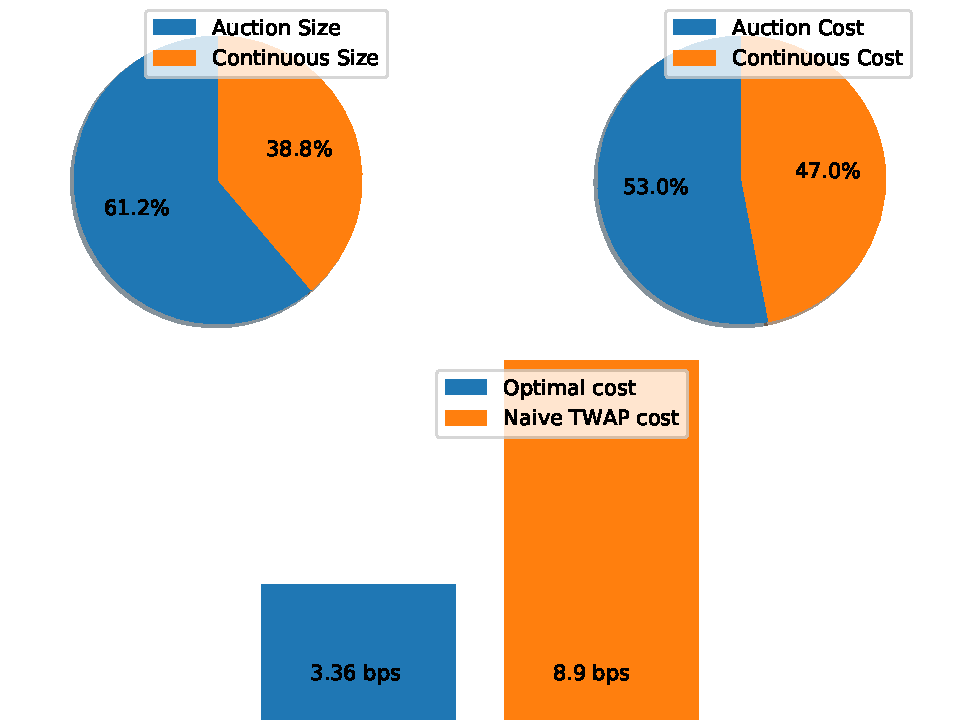
\includegraphics[width=\textwidth]{SampleTradeSize}
  \caption{Sample allocation between auction's block trade and the continuous trading strategy's size, using data from stock ACGL in October 2019, trading 5 percents of average trading volume of the first half of trading day. Compared to a pure TWAP trading stategy, the optimal stategy allocates 61.19 percents of the total position to be executed during the auction phase. The cost of trading in the auction phase accounts for 53.00 percents of the total cost of the strategy, while reducing 62.26 percents of total cost compared to a pure TWAP strategy, from 8.90 bps per share to 3.36 bps per share.}
  \label{fig:optimal_sizes}
\end{figure}



\begin{figure}[h]
  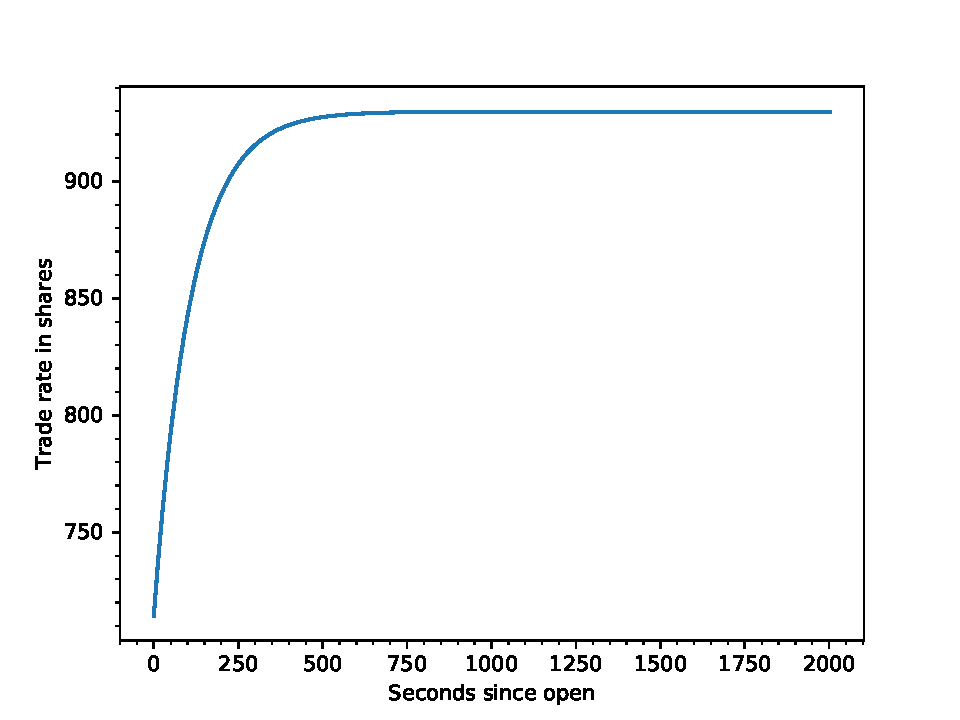
\includegraphics[width=\textwidth]{images/SampleTradeCurve}
  \caption{Sample optimal trading strategy's execution curve 30 minutes after market opens from auction phase. The shape of the optimal trading curve reflects the nature of the cost, in which the rate of execution is speed up over time as the market impact of the auction subsidizing and the spread narrowing.}
  \label{fig:optimal_curve_strategy}
\end{figure}

{\color{red}
\subsubsection{Optimal trading strategy under risk-aversion setting}

While the call auction represents an additional source of liquidity to lower overall trading cost, it is not the only benefit of trading in a call auction. Due to the fact that the call auction consolidate order flow over a period of time to a single price and point in time, a risk averse trader will be more likely to increase his execution size during the call auction compared to the continuous trading phase.

Let assume 
\begin{itemize}
  \item $\sigma$ is the volatility of the price process during continuous trading phase.
  \item $\gamma$ is the risk aversion factor of the liquidity trader.
\end{itemize}

Under the mean-variance optimization, we have the objective functional is:
\[
  J(ts) = \alpha \nu^2 + \frac{\alpha (\nu + \bar{V_e})}{2} \int_0^t e^{-\rho t} \xi(s) ds + \beta \int_0^t \xi(s)^2 ds + \gamma \int_0^t \Xi(s)^s
\]
Based on the Proof (\ref{proof:optimal-strategy-mixed-auction}), we have the optimal size of the block trader, taken into account the risk aversion factor, is:
\[
\nu = \frac{x_0 E_{11} + V_e E_{12} + E_{13}}{E_2}
\]
where the constants $E_{11}$, $E_{12}$, $E_{13}$ and $E_2$ are defined in the Appendix. The optimal trading strategy during continuous trading phase is then:
\begin{eqnarray*}
  \Xi(t) &=& C_1 e^{k t} + C_2 e^{-k t} + C_3 e^{-\rho t} \\
  \xi(t) &=& C_1 k e^{k t} - C_2 k e^{-k t} - C_3 \rho e^{-\rho t} 
\end{eqnarray*}
where $k=\sqrt{\frac{\gamma \sigma^2}{2\beta}}$ and the constants $C_1$, $C_2$ and $C_3$ are defined in the Appendix.

For illustration, we first compare the trading rate of the optimal trading strategy with the classical TWAP trading curve of Almgren-Chriss in Figure (\ref{fig:trading_rate_comparison}). We can see that the optimal trading strategy's position curve is steeper than the classical Almgren-Chriss's solution. This is due to the fact that the curvature of the optimal trading strategy's curve is determined by two factors: the risk aversion level of the trader and the exponential decays of the spread cost from auction matching. 

On the other hand, the risk aversion factor also affects the allocation of the optimal trading size during auction. We plot the auction size percentage of the whole portfolio in Figure (\ref{fig:auction_size_pct}). We can see that as expected volatility increases, the optimal trading strategy will allocate more into the auction to avoid exposure to volatility during trading phase, and vice versa.

\begin{figure}
	\centering
	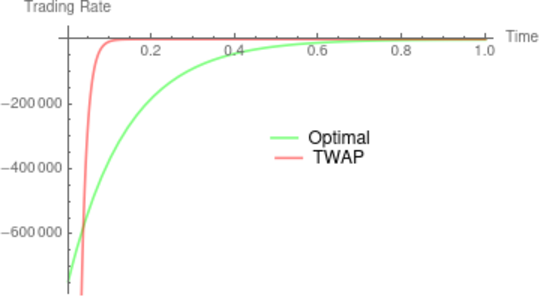
\includegraphics[width=7.5cm]{images/ContinuousTradingRate}
	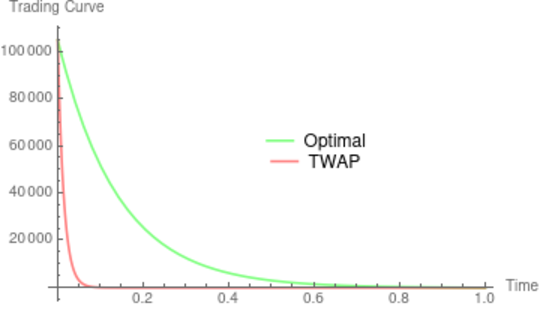
\includegraphics[width=7.5cm]{images/ContinuousTradingCurve}
	\caption{Trading rate (left) and position residual (right) comparison between the optimal trading strategy and the TWAP from Almgren-Chriss strategy. }
	\label{fig:trading_rate_comparison}
\end{figure}
\begin{figure}
	\centering
	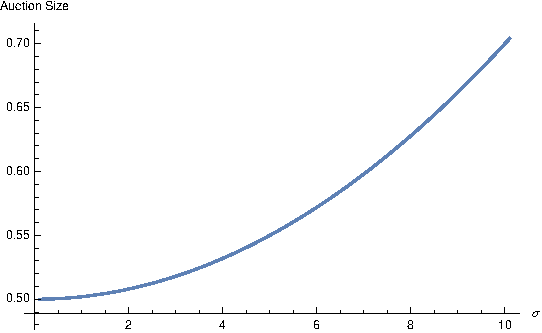
\includegraphics[width=15cm]{images/AuctionSizePct}
	\caption{Percentage of auction trading in the total portfolio against increase in expected volatility. The higher the expected volatility, the higher the percentage of the whole portfolio is allocated to be executed in the call auction.}
	\label{fig:auction_size_pct}
\end{figure}
}
\subsection{Summary}

The main findings of this section can be summarized as follows:

\begin{itemize}
  \item The presence of informed trading from the market maker is required for the transition to continuous trading, as the market maker will provide the necessary liquidity to offset the buy-sell imbalance at the end of the call auction.
  \item The transition period from the call auction will be characterized with a wide initial spread narrowing over time due to inventory management from the market maker, as shown in Equation (\ref{eqn:cost_equation_all}).
  \item Trading in the call auction lower the total execution cost compared to trading in continuous auction only, as the call auction provides an additional venue for liquidity consumption.
  \item There is an optimal liquidation strategy to execute trade during both the call auction and the continuous auction. The mixing ratio of the strategy is determined by the efficiency of each auction, in terms of immediate cost of aggressing the book and the speed of spread recovery after market opening.
  \item {\color{red}Trading in the call auction has the potential benefit of reducing the total variance of the execution. Given the risk aversion factor, a liquidity trader will increase his trading size during the call auction in his optimal trading strategy in proportion to the expected volatility and/or his risk aversion factor.}
\end{itemize}

Before moving to empirical analysis, it is imperative to address some stylized facts of our model. We assume that the liquidity traders are price takers who submit market orders to signify his intention to trade regardless of opening price, and the market maker will post limit orders to counter the imbalance. In most modern stock exchanges, all participants can post limit orders in the order book to be "crossed" during the opening match. Limit orders can also be modified or cancelled before the opening match, allowing participants to update their pricing. However, as long as the market maker in our model can place his trade after all the liquidity traders has submitted their orders, the pricing schedule based on the market imbalance still holds.

We also assume that there is only one market maker and only he or she trades with private information. In practice, there can be multiple agents trading with information. However, as long as the private information is derived from public data, that is, no insider trading, we can assume that all informed agent will have the same "signal" regarding the fair price of the stock, and are only different in their risk aversion factor. Therefore, we can assume that all informed agents are trading with same risk aversion factor, which are represented by the market maker in our model. The principal agent who provides liquidity in the call auction is assumed to be a market maker because, as shown in our model, he will need to make a spread in the continuous auction to capture the expected profit from his signal.

The source of private information is also a vital assumption in our model. We assume that the market maker derives his valuation from public information, which include, but not limited to, the following factors:

\begin{itemize}
  \item Public order flow, with or without identity.
  \item General market information, such as index futures movement before equity market opening.
  \item Price continuity from previous day's closing price. In absence of any fundamental news, it is reasonable to expect the opening price to be close to the previous day's closing price.
\end{itemize}

Another deviation is the inventory management effects of the market maker. In our model, there is market maker's inventory management effects on the spread due to the position acquired from the opening auction, but not in the continuous auction. While it would be more complete to account for the inventory management effects in both auctions, our empirical analysis suggests that the inventory management effects of the continuous auction is less prominent compared to the opening auction. Specifically, we observed that

\begin{itemize}
  \item There is little evidence that the bid-ask spread is changed following a trade except near the opening and closing auctions.
  \item The auction matching volume is usually much larger than a normal trade during continuous phase, accounted for a significant fraction of the daily trading volume.
\end{itemize}

Last but not least, although it is immaterial to our cost analysis, it is not obvious that the market maker will be profitable after placing his "stabilization" trade to counter the opening auction's imbalance. Even when his initial signal is correct up to the end of the opening auction, new information may come and he has to change his valuation of the stock before realize the signal from the call auction. This is evident in the high volatility immediately after market opening. However, the continuous book is only one of many execution venue for the market maker to realize his signal. For example, the market maker may attempt to "lock-in" his profit by hedging into the index futures immediately. He then can slowly unwind both legs of the hedge over the course of the day, resulting in a tightening spread over time.

With those caveats in mind, we can proceed to the empirical analysis of NASDAQ data to estimate the liquidation cost of trading in both auctions compared to only during the continuous auction.